\documentclass{ximera}

%\usepackage{todonotes}

\newcommand{\todo}{}

\usepackage{esint} % for \oiint
\graphicspath{
  {./}
  {ximeraTutorial/}
}

\newcommand{\mooculus}{\textsf{\textbf{MOOC}\textnormal{\textsf{ULUS}}}}

\usepackage{tkz-euclide}
\tikzset{>=stealth} %% cool arrow head
\tikzset{shorten <>/.style={ shorten >=#1, shorten <=#1 } } %% allows shorter vectors

\usetikzlibrary{backgrounds} %% for boxes around graphs
\usetikzlibrary{shapes,positioning}  %% Clouds and stars
\usetikzlibrary{matrix} %% for matrix
\usepgfplotslibrary{polar} %% for polar plots
\usetkzobj{all}
\usepackage[makeroom]{cancel} %% for strike outs
%\usepackage{mathtools} %% for pretty underbrace % Breaks Ximera
\usepackage{multicol}
\usepackage{pgffor} %% required for integral for loops


%% http://tex.stackexchange.com/questions/66490/drawing-a-tikz-arc-specifying-the-center
%% Draws beach ball 
\tikzset{pics/carc/.style args={#1:#2:#3}{code={\draw[pic actions] (#1:#3) arc(#1:#2:#3);}}}



\usepackage{array}
\setlength{\extrarowheight}{+.1cm}   
\newdimen\digitwidth
\settowidth\digitwidth{9}
\def\divrule#1#2{
\noalign{\moveright#1\digitwidth
\vbox{\hrule width#2\digitwidth}}}





\newcommand{\RR}{\mathbb R}
\newcommand{\R}{\mathbb R}
\newcommand{\N}{\mathbb N}
\newcommand{\Z}{\mathbb Z}

\newcommand{\sagemath}{\textsf{SageMath}}


%\renewcommand{\d}{\,d\!}
\renewcommand{\d}{\mathop{}\!d}
\newcommand{\dd}[2][]{\frac{\d #1}{\d #2}}
\newcommand{\pp}[2][]{\frac{\partial #1}{\partial #2}}
\renewcommand{\l}{\ell}
\newcommand{\ddx}{\frac{d}{\d x}}

\newcommand{\zeroOverZero}{\ensuremath{\boldsymbol{\tfrac{0}{0}}}}
\newcommand{\inftyOverInfty}{\ensuremath{\boldsymbol{\tfrac{\infty}{\infty}}}}
\newcommand{\zeroOverInfty}{\ensuremath{\boldsymbol{\tfrac{0}{\infty}}}}
\newcommand{\zeroTimesInfty}{\ensuremath{\small\boldsymbol{0\cdot \infty}}}
\newcommand{\inftyMinusInfty}{\ensuremath{\small\boldsymbol{\infty - \infty}}}
\newcommand{\oneToInfty}{\ensuremath{\boldsymbol{1^\infty}}}
\newcommand{\zeroToZero}{\ensuremath{\boldsymbol{0^0}}}
\newcommand{\inftyToZero}{\ensuremath{\boldsymbol{\infty^0}}}



\newcommand{\numOverZero}{\ensuremath{\boldsymbol{\tfrac{\#}{0}}}}
\newcommand{\dfn}{\textbf}
%\newcommand{\unit}{\,\mathrm}
\newcommand{\unit}{\mathop{}\!\mathrm}
\newcommand{\eval}[1]{\bigg[ #1 \bigg]}
\newcommand{\seq}[1]{\left( #1 \right)}
\renewcommand{\epsilon}{\varepsilon}
\renewcommand{\phi}{\varphi}


\renewcommand{\iff}{\Leftrightarrow}

\DeclareMathOperator{\arccot}{arccot}
\DeclareMathOperator{\arcsec}{arcsec}
\DeclareMathOperator{\arccsc}{arccsc}
\DeclareMathOperator{\si}{Si}
\DeclareMathOperator{\proj}{\vec{proj}}
\DeclareMathOperator{\scal}{scal}
\DeclareMathOperator{\sign}{sign}


%% \newcommand{\tightoverset}[2]{% for arrow vec
%%   \mathop{#2}\limits^{\vbox to -.5ex{\kern-0.75ex\hbox{$#1$}\vss}}}
\newcommand{\arrowvec}{\overrightarrow}
%\renewcommand{\vec}[1]{\arrowvec{\mathbf{#1}}}
\renewcommand{\vec}{\mathbf}
\newcommand{\veci}{{\boldsymbol{\hat{\imath}}}}
\newcommand{\vecj}{{\boldsymbol{\hat{\jmath}}}}
\newcommand{\veck}{{\boldsymbol{\hat{k}}}}
\newcommand{\vecl}{\boldsymbol{\l}}
\newcommand{\uvec}[1]{\mathbf{\hat{#1}}}
\newcommand{\utan}{\mathbf{\hat{t}}}
\newcommand{\unormal}{\mathbf{\hat{n}}}
\newcommand{\ubinormal}{\mathbf{\hat{b}}}

\newcommand{\dotp}{\bullet}
\newcommand{\cross}{\boldsymbol\times}
\newcommand{\grad}{\boldsymbol\nabla}
\newcommand{\divergence}{\grad\dotp}
\newcommand{\curl}{\grad\cross}
%\DeclareMathOperator{\divergence}{divergence}
%\DeclareMathOperator{\curl}[1]{\grad\cross #1}
\newcommand{\lto}{\mathop{\longrightarrow\,}\limits}

\renewcommand{\bar}{\overline}

\colorlet{textColor}{black} 
\colorlet{background}{white}
\colorlet{penColor}{blue!50!black} % Color of a curve in a plot
\colorlet{penColor2}{red!50!black}% Color of a curve in a plot
\colorlet{penColor3}{red!50!blue} % Color of a curve in a plot
\colorlet{penColor4}{green!50!black} % Color of a curve in a plot
\colorlet{penColor5}{orange!80!black} % Color of a curve in a plot
\colorlet{penColor6}{yellow!70!black} % Color of a curve in a plot
\colorlet{fill1}{penColor!20} % Color of fill in a plot
\colorlet{fill2}{penColor2!20} % Color of fill in a plot
\colorlet{fillp}{fill1} % Color of positive area
\colorlet{filln}{penColor2!20} % Color of negative area
\colorlet{fill3}{penColor3!20} % Fill
\colorlet{fill4}{penColor4!20} % Fill
\colorlet{fill5}{penColor5!20} % Fill
\colorlet{gridColor}{gray!50} % Color of grid in a plot

\newcommand{\surfaceColor}{violet}
\newcommand{\surfaceColorTwo}{redyellow}
\newcommand{\sliceColor}{greenyellow}




\pgfmathdeclarefunction{gauss}{2}{% gives gaussian
  \pgfmathparse{1/(#2*sqrt(2*pi))*exp(-((x-#1)^2)/(2*#2^2))}%
}


%%%%%%%%%%%%%
%% Vectors
%%%%%%%%%%%%%

%% Simple horiz vectors
\renewcommand{\vector}[1]{\left\langle #1\right\rangle}


%% %% Complex Horiz Vectors with angle brackets
%% \makeatletter
%% \renewcommand{\vector}[2][ , ]{\left\langle%
%%   \def\nextitem{\def\nextitem{#1}}%
%%   \@for \el:=#2\do{\nextitem\el}\right\rangle%
%% }
%% \makeatother

%% %% Vertical Vectors
%% \def\vector#1{\begin{bmatrix}\vecListA#1,,\end{bmatrix}}
%% \def\vecListA#1,{\if,#1,\else #1\cr \expandafter \vecListA \fi}

%%%%%%%%%%%%%
%% End of vectors
%%%%%%%%%%%%%

%\newcommand{\fullwidth}{}
%\newcommand{\normalwidth}{}



%% makes a snazzy t-chart for evaluating functions
%\newenvironment{tchart}{\rowcolors{2}{}{background!90!textColor}\array}{\endarray}

%%This is to help with formatting on future title pages.
\newenvironment{sectionOutcomes}{}{} 



%% Flowchart stuff
%\tikzstyle{startstop} = [rectangle, rounded corners, minimum width=3cm, minimum height=1cm,text centered, draw=black]
%\tikzstyle{question} = [rectangle, minimum width=3cm, minimum height=1cm, text centered, draw=black]
%\tikzstyle{decision} = [trapezium, trapezium left angle=70, trapezium right angle=110, minimum width=3cm, minimum height=1cm, text centered, draw=black]
%\tikzstyle{question} = [rectangle, rounded corners, minimum width=3cm, minimum height=1cm,text centered, draw=black]
%\tikzstyle{process} = [rectangle, minimum width=3cm, minimum height=1cm, text centered, draw=black]
%\tikzstyle{decision} = [trapezium, trapezium left angle=70, trapezium right angle=110, minimum width=3cm, minimum height=1cm, text centered, draw=black]




\outcome{Identify pairs in a relation.}


\begin{document}

\begin{definition}
  During the annual Totman reunion, a group from the Totman family played badminton. The map below identifies the pairs in the \textbf{Badminton} function.
  
  

    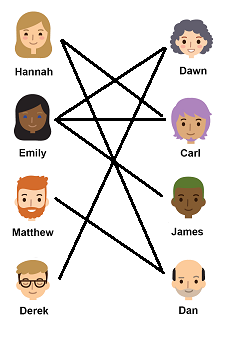
\includegraphics[width=245px,height=352px]{pics/badminton.png}

  
 

  The \dfn{Badminton} relation includes three sets:
    \begin{itemize}
    \item A first set consisting of 8 family members identified in the map.
    \item A second set consisting of the same 8 family members identified in the map.
    \item A set of ordered pairs. The pair (first person, second person) is a member of the Badminton relation if the first person and the second person played each other in a Badminton game.
    \end{itemize}

  
\end{definition}



\begin{exercise}
 ({
\includegraphics[width=50px,height=65px]{pics/people/emily.png}}, {
\includegraphics[width=50px,height=65px]{pics/people/dan.png}}) $\in$ Badminton 

  \begin{multipleChoice}
    \choice{True}
    \choice[correct]{False}
  \end{multipleChoice}
  \begin{feedback}
The map does not connect Emily and Dan.
  \end{feedback}
\end{exercise}












\begin{exercise}
How many Badminton games were played? $\answer{7}$
  \begin{feedback}
Each line in the map represents a game.
  \end{feedback}
\end{exercise}




\begin{exercise}
How many pairs are in the Badminton relation? $\answer{14}$
  \begin{feedback}
Each line in the map represents two pairs.
  \end{feedback}
\end{exercise}





\begin{definition}
The Badminton group decided to form two teams and play a Badminton match. The map below identifies the pairs in the \textbf{TeamBadminton} function.
  
  

    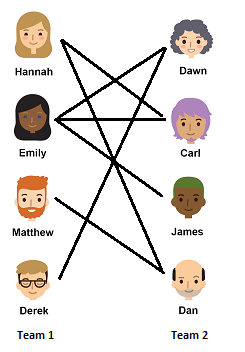
\includegraphics[width=245px,height=352px]{pics/badminton2.png}

  
 

  The \dfn{TeamBadminton} relation includes three sets:
    \begin{itemize}
    \item A first set, called Team 1, consisting of 4 family members identified in the map.
    \item A second set , called Team 2, consisting of 4 family members identified in the map.
    \item A set of family ordered pairs. The pair (first person, second person) is a member of the TeamBadminton relation  provided
            \begin{itemize}
            \item person1 is on Team 1.
            \item person2 is on Team 2.
            \item person1 played person2 is a game of Badminton.
            \end{itemize}

    \end{itemize}

  
\end{definition}










\begin{exercise}

 ({
\includegraphics[width=50px,height=65px]{pics/people/dawn.png}}, {
\includegraphics[width=50px,height=65px]{pics/people/derek.png}}) $\in$ TeamBadminton 

  \begin{multipleChoice}
    \choice{True}
    \choice[correct]{False}
  \end{multipleChoice}
  \begin{feedback}
Derek is on Team 1 and would need to be listed first in the pair.
  \end{feedback}
\end{exercise}





\begin{exercise}



 ({
\includegraphics[width=50px,height=65px]{pics/people/emily.png}}, {
\includegraphics[width=50px,height=65px]{pics/people/james.png}}) $\in$ TeamBadminton 

  \begin{multipleChoice}
    \choice[correct]{True}
    \choice{False}
  \end{multipleChoice}
  \begin{feedback}
Emily is on Team 1. James is on Team 2.  They played a game of Badminton.
  \end{feedback}
\end{exercise}



\begin{exercise}
Is TeamBadminton reflexive?

  \begin{multipleChoice}
    \choice{Yes}
    \choice[correct]{No}
  \end{multipleChoice}
  \begin{feedback}
A person is not on both Team 1 and Team 2.
  \end{feedback}
\end{exercise}




\begin{exercise}
Is TeamBadminton symmetric?

  \begin{multipleChoice}
    \choice{Yes}
    \choice[correct]{No}
  \end{multipleChoice}
  \begin{feedback}
  If (person1, person2) is in TeamBadminton, then person1 is on Team 1, therefore the pair (person2, person1) cannot be in TeamBadminton.
  \end{feedback}
\end{exercise}





\begin{exercise}
Is TeamBadminton transitive?

  \begin{multipleChoice}
    \choice[correct]{Yes}
    \choice{No}
  \end{multipleChoice}
  \begin{feedback}
If (person1, person2) is in TeamBadminton, then (person2, person3) cannot be in TeamBadminton.  That means there is not situation where both (person1, person2) and (person2, person3) are in TeamBadminton.  This mens there is no way to violate the transitive definition.  The transitive definition is automatically valid.
  \end{feedback}
\end{exercise}




\begin{exercise}
How many solutions are there to the following statement?  

({
\includegraphics[width=50px,height=65px]{pics/people/hannah.png}}, PERSON) $\in$ TeamBadminton 

\[  \answer{2} \]

  \begin{feedback}
Hannah played Carl and Dan from Team 2.
  \end{feedback}
\end{exercise}





\begin{exercise}
How many solutions are there to the following statement?  

(PERSON, {\includegraphics[width=50px,height=65px]{pics/people/Matthew.png}} ) $\in$ TeamBadminton 

\[  \answer{0} \]

  \begin{feedback}
Matthew is on Team 1 and cannot be in the second position of a pair.
  \end{feedback}
\end{exercise}







\end{document}
